% #############################################################################
% This is Chapter 1
% !TEX root = ../main.tex
% #############################################################################
% Change the Name of the Chapter i the following line
\fancychapter{Introduction}
\cleardoublepage
% The following line allows to ref this chapter
\label{chap:intro}


In this thesis proposal, we address the critical environmental challenge of accurately monitoring methane emissions, a task vital in the fight against climate change. Methane, being a key greenhouse gas, commands attention in climate policy due to its significant role in global warming. Our approach, innovatively combining Causal Machine Learning (CML) with Generative AI in satellite imagery analysis, aims to revolutionize methane emission surveillance. This integration seeks to advance beyond the traditional machine learning methodologies that often fall short in capturing the complex, causal dynamics behind methane emissions.

CML steps into this gap, offering an in-depth understanding of cause-effect relationships vital for attributing emissions accurately. This capability is essential, not just for scientific understanding but also for shaping informed policy decisions and pinpointing liability in the context of environmental regulations. By employing Generative AI, specifically through Generative Adversarial Networks (GANs), we enhance this approach further. This technology enables the generation of synthetic satellite imagery, simulating a vast array of environmental scenarios, including those rare or extreme conditions that are typically underrepresented. Such enriched datasets are crucial for developing adaptable models that can interpret diverse environmental phenomena.

However, the journey of integrating CML with Generative AI is intricate and demanding. The process of discerning true causal links from the complex mosaic of satellite data requires a harmonious blend of advanced computational techniques and multidisciplinary knowledge. While CML provides a pathway to deeper insights and interpretability, Generative AI brings in the dimension of data diversity and experimentation without the constraints of real-world data collection.

This research aims to harness the strengths of both CML and Generative AI to create a robust and adaptable framework for methane emission monitoring. Our objectives are not limited to technical advancements; we also aim to offer new perspectives for understanding the interactions between methane emissions and environmental changes. Ultimately, this proposal is poised to make a significant contribution to environmental monitoring, policy-making, and our broader understanding of climate dynamics.

The vigilant monitoring of methane emissions is a cornerstone in the global strategy against climate change. Methane, notorious for its potent greenhouse effect, presents a unique challenge for scientists and policymakers alike. As countries mobilize to meet climate goals, the need for precise quantification and attribution of these emissions becomes ever more crucial. This is not just a matter of scientific inquiry but a pressing issue that intersects with climate policy and legal frameworks, where accuracy in monitoring can influence regulatory outcomes and determine liability.

At the core of this thesis is the proposition to leverage the strengths of Causal Machine Learning (CML) and Generative AI to refine the current capabilities of satellite-based methane emission monitoring. This integration is anticipated to revolutionize the field by providing enhanced precision, greater interpretability, and the ability to simulate diverse environmental scenarios, which are essential for robust policy-making and establishing accountability.


\section{Justification}

Methane, a colorless and odorless gas, plays a critical role in various Earth's atmospheric processes, notably global warming. Its prominence as the second most significant contributor to post-industrial global warming, after carbon dioxide, is underscored by a Global Warming Potential (GWP) 28-34 times that of CO2 over a century \cite{tian_catalytic_2021, IPCC2013}. Its major source, wetland methane emissions, constitutes about 20-30\% of global emissions, making it a significant focus for climate change mitigation efforts \cite{bousquet_contribution_2006, chen_estimation_2006}.

Given methane's abundance and lower cost compared to other fuels, it emerges as an economically viable energy source. However, the technical challenges in capturing and storing methane, due to its gaseous nature at standard temperature and pressure, necessitate innovative approaches \cite{cardenas_is_1996, rajnauth_monetizing_2008}. These challenges, coupled with methane's potential as a cleaner-burning fuel, highlight the need for continued research and development in effective methane utilization technologies.

Global methane emissions, estimated at approximately 570 million tonnes annually, have seen a recent increase of 9.8\% between 2018-2019 \cite{stocker2014climate, friedlingstein2020global}. Addressing this uptick, the International Methane Emissions Observatory (IMEO) was established to support the Global Methane Pledge's goal of reducing methane emissions in key sectors by 30\% by 2030.

Satellite-based systems have been instrumental in detecting major methane emission events, facilitating mitigation efforts and tracking progress \cite{eo_portal_iss_2023, eo_portal_copernicus_2012, eo_portal_gosat_gw_2023, ghgsat_ghgsat_2023, writer_methane_tracking_2023}. Advances in technology, particularly the use of machine learning approaches, have further enhanced the detection of methane emissions from satellite imagery \cite{irakulis_loitxate_satellites_2022, maasakkers_using_2022, sherwin_single_blind_2023, joyce_using_2023, Prasad2020, wu2020deep, kumar_deep_2020}.

However, the complexity of detecting and quantifying methane emissions from satellite images calls for sophisticated machine learning algorithms. This need coincides with the growing demand within the machine learning community for models that are not only effective but also transparent and interpretable \cite{roscher_explainable_2020, hall_review_2022}.

Causal learning, a subset of machine learning focused on understanding cause-effect relationships, represents a paradigm shift from traditional statistical analysis. This approach has seen applications in various domains, including healthcare, where it aids in decision-making and estimating intervention impacts \cite{pearl_causal_2009, verboven_combining_2022, subramanian_estimating_2023, otgonbaatar_causality_2022, angell_estimating_2021, osazuwa_ness_causal_2022}. In methane detection from satellite images, causal learning can enhance the accuracy and reliability of algorithms by unraveling causal relationships between various factors in satellite imagery and methane emissions. This approach allows for the development of models that are not only robust and generalizable but also interpretable, a crucial attribute for ensuring accountability and transparency.

The primary objective of this research is to harness causal learning in detecting methane emissions from satellite images. This endeavor is driven by the urgent necessity to accurately monitor and mitigate methane emissions as a strategy against climate change. The novelty of applying causal learning in this field presents a unique opportunity for significant contributions to both methane detection and the broader domain of causal learning.

Our proposed methodology involves applying causal learning techniques to satellite imagery to discern the causes and effects of methane emissions globally. Causal learning, which focuses on deciphering causal relationships between variables, is adept at addressing complex and multidimensional data sets like those obtained from satellite imagery. It enables us to answer counterfactual queries, assess policy optimization, and examine the robustness and biases in models. By leveraging data from satellite missions like WorldView-3 and Landsat 8, which offer multispectral and high-resolution images, we can obtain comprehensive and frequent global coverage. This facilitates the detection and monitoring of methane emissions in otherwise inaccessible areas, as well as the study of their temporal and spatial dynamics.

The causal learning techniques we plan to use include Bayesian networks, causal trees, and structural graphical models. These techniques have been successfully applied in various fields but are relatively nascent in remote sensing. Our work aims to improve scientific understanding of the methane cycle and support informed decision-making for its mitigation. We also anticipate this research to offer insights into methane emission policies and regulations, aiding in the development of effective and equitable strategies to reduce the global methane footprint and promote sustainable development.



%%%%%%%





\section{Review of Relevant Literature}
Key papers were reviewed and synthesized to underpin the research on integrating Causal Machine Learning (CML) with Generative AI for methane emission monitoring using satellite imagery.

The evolution of causal inference methodologies and their application in diverse fields, particularly in environmental monitoring using satellite imagery, forms the cornerstone of this thesis. This research stands at the confluence of several pioneering studies, each contributing unique perspectives and methodological insights vital for understanding methane emissions.

The work of Cheong et al. \cite{cheong2023} is particularly instructive in its use of structural causal models (SCMs) for bias identification in affect recognition. While their application domain focuses on facial affect recognition, the underlying principles of utilizing SCMs for unraveling complex causal relationships are highly relevant. This methodology parallels the challenges faced in dissecting the causal mechanisms underlying methane emissions as observed through satellite data, where biases and confounding factors can significantly influence interpretation and conclusions.

Cheng and Redfern’s exploration into quantifying causal contributions in Earth systems \cite{cheng2021} also bears significant relevance. Their innovative use of normalized information flow (nIFc) to address high-dimensional and intricate data systems mirrors the complexities encountered in analyzing satellite-based methane emission data. Their approach exemplifies the nuanced understanding required to decode intricate causal relationships from large-scale environmental data.

Additionally, Jerzak et al.'s \cite{jerzak2023} integration of earth observation data into causal inference directly aligns with the central aims of this thesis. Their methodological advancements provide a critical framework for leveraging satellite imagery in causal analysis. This study serves as a guidepost for employing remote sensing data in understanding causality in environmental contexts, especially in examining how different factors influence methane emission patterns.

Moreover, the application of machine learning in methane emissions mitigation, as demonstrated by Wang et al. \cite{wang2020}, offers practical insights into the use of advanced analytics in environmental monitoring. Their work underscores the potential of machine learning techniques in enhancing the detection and analysis of methane emissions, a concept that is central to this thesis. The methodologies and findings from their research in identifying methane super-emitters in the oil and gas industry provide valuable perspectives on how satellite data, coupled with machine learning algorithms, can be harnessed for more effective environmental monitoring.


In \textit{LEARNING INVARIANT REPRESENTATIONS FOR REINFORCEMENT LEARNING WITHOUT RECONSTRUCTION} \cite{zhang_learning_2021}, the authors present a novel approach to representation learning for reinforcement learning, focusing on bisimulation metrics to capture behavioral similarity in continuous Markov Decision Processes (MDPs). This work is pivotal for your research as it emphasizes learning representations that are invariant to task-irrelevant details, a concept crucial when analyzing methane emissions from satellite imagery where irrelevant environmental factors must be distinguished from relevant methane emission indicators. Figure 3 from their work \cite[Figure 3]{zhang_learning_2021}, demonstrates the effectiveness of their method in disregarding task-irrelevant information, which could be analogous to filtering out irrelevant geographical features in satellite imagery for methane monitoring.

\textit{CA-SpaceNet: Counterfactual Analysis Framework for 6D Pose Estimation of Space-Borne Targets} \cite{wang_ca-spacenet_2022} introduces the CA-SpaceNet framework, employing counterfactual analysis for robust 6D pose estimation of space objects in complex backgrounds. The adoption of causal inference in this context, particularly the methodology to reduce side effects caused by background interference (as shown in their network architecture, Figure 2 \cite[Figure 2]{wang_ca-spacenet_2022}), provides insights into handling confounding factors in satellite imagery, a significant concern in accurately identifying methane emission sources.

\textit{Integrating Earth Observation Data into Causal Inference: Challenges and Opportunities} by Jerzak et al. \cite{jerzak_integrating_2023} directly aligns with the theme of your thesis. They focus on the use of satellite imagery as a proxy for confounders in observational studies, particularly in settings with sparse data, such as developing countries. This paper provides methodological guidance for causal estimation when confounding is induced by patterns or objects observed in images, which is fundamental to your research. Table 1 in their work \cite[Table 1]{jerzak_integrating_2023} offers a comprehensive comparison of satellite imagery with other data types in observational causal inference, which could be highly relevant for contextualizing your methodology. This study of scene-based confounding in \cite{jerzak_integrating_2023} offers an in-depth understanding of how treatment, outcome, and confounder can be defined at different scales in satellite imagery, allowing for more nuanced analysis. This aspect is particularly relevant for your research, where methane emission sources might be identified at different resolutions than the environmental impact they cause.

In the realm of estimation and interpretation in satellite image-based observational inference, provide valuable insights. They discuss the challenges and potential of satellite data for causal inference, highlighting the need for high-resolution imagery and robust model specification. This is especially pertinent to your thesis, as methane emission detection would require high-resolution satellite data to accurately identify emission hotspots.

Furthermore, the simulation studies in \cite{jerzak_integrating_2023} provide a practical framework for understanding the dynamics of observational inference with satellite images. The comparison of different estimators and the analysis of model misspecification can guide your approach to estimating the impact of methane emissions. Figure 4 from their paper \cite[Figure 4]{jerzak_integrating_2023} illustrates the relationship between kernel width, resolution scaling, and bias in the estimation, offering a valuable reference for your analysis.

These studies collectively chart the course for this research, each contributing essential elements to the framework of causal analysis in the context of methane emissions from satellite imagery. They not only inform the methodological approach of this thesis but also illuminate the interdisciplinary nature of research at the intersection of environmental science, causal inference, and satellite imaging.


%%%%%

%%%%%

% \noindent \todo[color=green!40,author=Rui Cruz, inline]{The examples of techniques, tools, and packages along the document are for you to get familiarized with them. It is advisable to preserve those examples of usage, for reference, by moving the respective blocks of text to the last Chapter of this template (or to a Chapter file that you know you will not use), until you finish your document.}

% \textcolor{violet}{Example of using package} \verb:todo: \textcolor{violet}{for notes of authors.} \textcolor{violet}{In this case} \todo[color=yellow!40,author=Johnny, fancyline]{pointing out to the place} \textcolor{violet}{the author Johnny is calling the attention for something at the specific place in the text.}

% \textcolor{violet}{In this other case, another co-author is commenting on something inline.} \todo[color=orange!40,author=Manuel, inline]{Inline comment or Note. It can be an extract of some recommended text. ``Lorem ipsum dolor sit amet, consectetuer adipiscing elit. Morbi commodo, ipsum sed pharetra gravida, orci magna rhoncus neque, id pulvinar odio lorem non turpis. Nullam sit amet enim. Suspendisse id velit vitae ligula volutpat condimentum. Aliquam erat volutpat. Sed quis velit. Nulla facilisi. Nulla libero. Vivamus pharetra posuere sapien.''}

% \textcolor{violet}{In this other case, another co-author is making a note about the citation for missing some bibliographic record}~\cite{Apple:2011fk,AdobeHDS:ys,A.:qy}.
% \todo[color=red!40,author=Pete]{You should cite also Pellentesque:2014}


% Nam consectetuer. Sed aliquam, nunc eget euismod ullamcorper, lectus nunc ullamcorper orci, fermentum bibendum enim nibh eget ipsum. Donec porttitor ligula eu dolor. Maecenas vitae nulla consequat libero cursus venenatis. Nam magna enim, accumsan eu, blandit sed, blandit a, eros.

% Quisque facilisis erat a dui. Nam malesuada ornare dolor. \enquote{Cras gravida, diam sit amet rhoncus ornare, erat elit consectetuer erat, id egestas pede nibh eget odio.}\todo[color=green!40,author=Rui Cruz, fancyline]{notice here how to enquote correctly}{} 

% Proin tincidunt, velit vel porta elementum, magna diam molestie sapien, non aliquet massa pede eu diam. Aliquam iaculis. Fusce et ipsum et nulla tristique facilisis. Donec eget sem sit amet ligula viverra gravida. Etiam vehicula urna vel turpis. Suspendisse sagittis ante a urna. Morbi a est quis orci consequat rutrum. Nullam egestas feugiat felis. Integer adipiscing semper ligula. Nunc molestie, nisl sit amet cursus convallis, sapien lectus pretium metus, vitae pretium enim wisi id lectus. Donec vestibulum. Etiam vel nibh. Nulla facilisi. Mauris pharetra. Donec augue. Fusce ultrices, neque id dignissim ultrices, tellus mauris dictum elit, vel lacinia enim metus eu nunc.

% \textcolor{violet}{This is an example of Tracking} \replaced[id=JO]{Changes}{Xanges} (in this case a replacement) by different authors in the document. The Text can additionally be modified by \added[id=PT]{adding} new text or by deleting \deleted[id=MN]{wrong} inadequate text. Author can manipulate changes \replaced[id=PT]{introduced by each author\deleted[id=MN]{, as adequate}}{intrroduced by other authors}.

% Proin at eros non eros adipiscing mollis. Donec semper turpis sed diam. Sed consequat ligula nec tortor. Integer eget sem. Ut vitae enim eu est vehicula gravida. Morbi ipsum ipsum, porta nec, tempor id, auctor vitae, purus. Pellentesque neque. Nulla luctus erat vitae libero. Integer nec enim. Phasellus aliquam enim et tortor. Quisque aliquet, quam elementum condimentum feugiat, tellus odio consectetuer wisi, vel nonummy sem neque in elit. Curabitur eleifend wisi iaculis ipsum.
% % #############################################################################
% \section{Morbi ipsum ipsum}
% Pellentesque nibh felis, eleifend id, commodo in, interdum vitae, leo. 
%  Praesent mauris \ac{SD} and \ac{HD} volutpat ligula eget enim \acp{WLAN} and 3G\slash 4G \acp{WWAN}.\todo[color=cyan!40, author=RC]{use of ACRONYM defined in file ``Thesis-MSc-Aconyms.tex''}

% Praesent eu elit. Ut eu ligula. Class aptent taciti sociosqu ad litora torquent per conubia nostra, per inceptos hymenaeos. Maecenas elementum augue nec nisl. Proin auctor lorem at nibh. Curabitur nulla purus, feugiat id, elementum in, lobortis quis, pede. Vivamus sodales adipiscing sapien.

% The use of Symbols in the document can be done using the Glossaries package, to display and also List them in the Indexes. 
% Praesent eu elit. Ut eu ligula. Class aptent taciti sociosqu ad litora torquent per conubia nostra, per inceptos hymenaeos. Maecenas elementum augue nec nisl. Proin auctor lorem at nibh. 

% For example, the initial diameter (\gls{diam0}) of the tube corresponds to a surface area (\gls{surfarea}) of $122 \mu{m}^2$.\todo[color=cyan!40, author=RC]{use of SYMBOL defined in file ``Thesis-MSc-Glossary.tex''}

% Praesent eu elit. Ut eu ligula. Class aptent taciti sociosqu ad litora torquent per conubia nostra, per inceptos hymenaeos. Maecenas elementum augue nec nisl. Proin auctor lorem at nibh. Curabitur nulla purus, feugiat id, elementum in, lobortis quis, pede. Vivamus sodales adipiscing sapien. Vestibulum posuere nulla eget wisi. Integer volutpat ligula eget enim. Suspendisse vitae arcu. Quisque pellentesque. Nullam consequat, sem vitae rhoncus tristique, mauris nulla fermentum est, bibendum ullamcorper sapien magna et quam. Sed dapibus vehicula odio. Proin bibendum gravida nisl. Fusce lorem. Phasellus sagittis, nulla in hendrerit laoreet, libero lacus feugiat urna, eget hendrerit pede magna vitae lorem. 
 
% Aliquam erat \ac{WLAN} volutpat \ac{CPU} mauris nulla fermentum est \ac{OS} Fusce magna mi, porttitor quis, convallis eget, sodales ac, urna.
% Pellentesque nibh felis, eleifend id, commodo in, interdum vitae, leo. Praesent eu elit. Ut eu ligula. Class aptent taciti sociosqu ad litora torquent per conubia nostra, per inceptos hymenaeos. Maecenas elementum augue nec nisl. Please notice the use of automatic referencig to objects such as Figures, Tables, equations, Algorithms, sections of a document, etc. by using the command \verb:\Cref{ref}: as in this case pointing to \Cref{fig:cashed}.\todo[color=cyan!40, author=RC, fancyline]{the correct Name of the float object, in this case a Figure, is determined by the system}

% \begin{figure}[htb]
% \centering
% 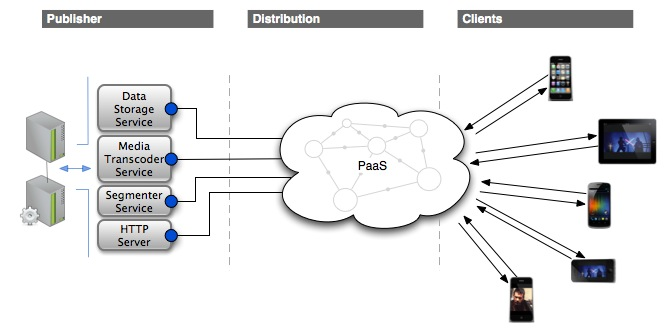
\includegraphics[width=0.9\textwidth]{./Images/cashed5}
% \caption{Ecosystem}
% \label{fig:cashed}
% \end{figure}

% Proin auctor lorem at nibh. Curabitur nulla purus, feugiat id, elementum in, lobortis quis, pede. Vivamus sodales adipiscing sapien. Vestibulum posuere nulla eget wisi. Integer volutpat ligula eget enim. Suspendisse vitae arcu. Quisque pellentesque. Nullam consequat, sem vitae rhoncus tristique, mauris nulla fermentum est, bibendum ullamcorper sapien magna et quam. Sed dapibus vehicula odio. Proin bibendum gravida nisl. Fusce lorem. Phasellus sagittis, nulla in hendrerit laoreet, libero lacus feugiat urna, eget hendrerit pede magna vitae lorem. Praesent mauris Class aptent taciti sociosqu ad litora torquent per conubia nostra, per inceptos hymenaeos H.264\slash \ac{AVC} standard, sem vitae rhoncus tristique \ac{SVC} \cite{Fraunhofer-Heinrich-Hertz-Institute:2013fk,ISO:H-264} nulla in hendrerit laoreet, libero lacus feugiat urna, eget hendrerit pede magna vitae lorem.

% \textcolor{violet}{You can use in-paragraph lists with this construct for: 
% \begin{inparaenum}[(a)]
% \item first case;
% \item second case; and
% \item third case,
% \end{inparaenum}
% making the text organized and fluid.}

% Vivamus auctor leo vel dui. Aliquam erat volutpat. Phasellus nibh. Vestibulum ante ipsum primis in faucibus orci luctus et ultrices posuere cubilia Curae; Cras tempor. Morbi egestas, urna non consequat tempus, nunc arcu mollis enim, eu aliquam erat nulla non nibh. Duis consectetuer malesuada velit. Nam ante nulla, interdum vel, tristique ac, condimentum non, tellus. Proin ornare feugiat nisl. Suspendisse dolor nisl, ultrices at, eleifend vel, consequat at, dolor, morbi egestas, urna non consequat tempus, nunc arcu mollis enim, eu aliquam erat nulla non nibh.

% Notice that \gls{maths} makes extensive use of \Glspl{formula}\todo[color=cyan!40, author=RC, fancyline]{example of use of Glossaries}{} which are particularly well rendered in documents produced with \gls{LaTeX}.

% Maecenas elementum augue nec nisl. Proin auctor lorem at nibh. Curabitur nulla purus, feugiat id, elementum in, lobortis quis, pede. Vivamus sodales adipiscing sapien. Vestibulum posuere nulla eget wisi. Integer volutpat ligula eget enim. Suspendisse vitae arcu. Quisque pellentesque.
% #############################################################################
% \section{Organization of the Document}
% This thesis is is organized as follows: \Cref{chap:intro} \todo[color=cyan!40, author=RC, fancyline]{references to doc sections/chapters are automatic}{}interdum vel, tristique ac, condimentum non, tellus. 
% In \cref{chap:back} curabitur nulla purus, feugiat id, elementum in, lobortis quis, pede.
% In \cref{chap:architecture} consequat ligula nec tortor. Integer eget sem. Ut vitae enim eu est vehicula gravida.
% \Cref{chap:implement} morbi egestas, urna non consequat tempus, nunc arcu mollis enim, eu aliquam erat nulla non nibh in \cref{chap:evaluation}.
% \Cref{chap:conclusion} suspendisse dolor nisl, ultrices at, eleifend vel, consequat at, dolor.